\chapter{Mô hình loại ảnh giao thông}
\section{Vấn đề và mục tiêu}
	Đối với vấn đề phát hiện kẹt xe qua hình ảnh camera, chúng ta sẽ sử dụng mạng neuron tích chập với tập ảnh huấn luyện được trích xuất từ những đoạn video do camera hành trình xe buýt ghi lại trong thời gian hoạt động. Ngoài ra, chúng ta còn sử dụng mô hình googLeNet để áp dụng vào vấn đề và phương pháp transfer learning (sẽ được trình bày trong mục tiếp theo). \par
\section{Phương pháp transfer learning}
	Ngày nay, với sự phát triển của Deep learning do nguồn dữ liệu to lớn và các máy tính ngày càng cải tiến về khả năng tính toán khiến cho kết quả chính xác của các bài toán phân loại ngày càng cao. Như mô hình mạng googLeNet có rất nhiều tầng khiến cho việc huấn luyện tốn kém thời gian. Thay vì như vậy chúng ta áp dụng phương pháp transfer learning.\par
	Transfer learning là công đoạn lấy model đã được huấn luyện tư một tập dữ liệu khác \cite{transfer} và tích hợp lại với tập dữ liệu có đang có. Việc này là khả thi do mô hình đã huấn luyện trước đó sử dụng tập ảnh khổng lồ giúp cho mồ hình học được loạt những đặc tính thường thấy trong cùng một ảnh. Có thể thấy tất cả các ảnh đều có những đặc tính cơ bản giống nhau, khi muốn huấn luyện lại cho tập ảnh của chính mình chúng ta chỉ cần thay tầng cuối cùng của mạng bằng tập dữ liệu của mình. Mô hình sẽ tự điều chỉnh lại các trọng số cũng như độ lệch từ các giá trị từ mô hình đã huấn luyện với tập dữ liệu mới mà không cần làm lại từ đầu.

\section{Các bước chuẩn bị}
\subsection{Tổng quan về tập dữ liệu}
	Để xây dựng mô hình phân loại hình ảnh, chúng ta cần phải có một tập huấn luyện đủ tốt. Ở đây, các hình ảnh được trích xuất từ camera hành trình từ các tuyến xe buýt. \par
	Cấu trúc tổ chức tập dữ liệu gồm 2 thư mục chính:
	\begin{itemize}
		\item Thư mục \textbf{ket}: chứa các hình ảnh được cho là giao thông trong tình trạng ùn tắt. Bao gồm 1077 hình ảnh định dạng JPG.
		\item Thư mục \textbf{thong}: chứa các hình ảnh được cho là giao thông trong tình trạng thông tháng. Bao gồm 2000 hình ảnh định dạng JPG.
	\end{itemize}

\subsection{Môi trường}
	Bộ phân loại ảnh giảo hông được huấn luyện trên nền tảng hệ điều hành Linux, ngôn ngữ Python phiên bản 3.6 kết hợp với thư viện Tensorflow mã nguồn mở chuyên được sử dụng cho những mô hình học sâu.\par
	Tensorflow\cite{tf} là một thư viện học sâu mã nguồn mở được Google phát triển. Thư viện này đã thu hút được sự chú ý lớn từ cộng đồng Deep-learning. Tensorflow cho phép chạy các thuật toán machine learning trên nhiều GPU, có nhiều module được dựng sẵn giúp cho việc xây dựng và thực thi mô hình đơn giản hơn. \par
	\textbf{Các khái niệm:}
	\begin{itemize}
		\item \textbf{Tensor:} đây là cấu trúc dữ liệu được sử dụng hoàn toàn trong Tensorflow. Hay nói cách khác, tất cả dữ liệu đều biểu diễn dưới dạng tensor. Đơn giản, tensor là một mảng gồm n chiều hay list kèm theo một số thuộc tính khác.
		
		\item \textbf{Rank:} còn được gọi là số chiều của dữ liệu
		\begin{table}[h!]
			\centering
			\begin{tabular}{ | c | c | c | }
 			\hline
 			 \textbf{Rank} & \textbf{Đơn vị số} & \textbf{Ví dụ}\\
 			\hline
 			0  & Scalar  & s = 123  \\
			\hline
			1 & Vector & s = [0.8, 0.1, 0.1]	\\
			\hline
			2 & Matrix & s = [[1,2,3], [4,5,6], [7,8,9]]	\\
			\hline
			3 & 3-Tensor & s = [ [ [1], [2], [3] ], [ [4], [5], [6] ], [ [7], [8], [9] ] ]	\\
			\hline
			n & n-Tensor & n chiều dữ liệu... \\
			\hline
			
		\end{tabular}
		\caption{Các chiều dữ liệu.}
		\label{table:rank}
		\end{table}
		
		
		
		
		\item \textbf{Shape:} biểu diễn chiều của tensor. Ví dụ, \(t = [[1,2,3], [4,5,6], [7,8,9]]\) có shape là \([3, 3]\), \(t = [ [ [1], [2], [3] ], [ [4], [5], [6] ], [ [7], [8], [9] ] ]\) có shape là \([1, 3, 3]\),...
		
		\item \textbf{Type:} là các kiểu dữ liệu được sử dụng trong Tensorflow. Một vài kiểu dữ liệu cơ bản như.\\
		\begin{table}[h!]
			\centering
			\begin{tabular}{ | c | c | c | }
 			\hline
 			 \textbf{Data type} & \textbf{Python code} & \textbf{Mô tả}\\
 			\hline
 			\textit{DT-FLOAT}  & tf.float32  & 32 bits floating point.  \\
			\hline
			\textit{DT-DOUBLE} & tf.float64 & 64 bits floating point.\\
			\hline
			\textit{DT-INT16} & tf.int16	 & 16 bits signed integer.\\
			\hline
			\textit{DT-INT32} & tf.int32	 & 32 bits signed integer.	\\
			\hline
			\textit{DT-INT64} & tf.int64	 & 64 bits signed integer. \\
			\hline
			... & ... & ...\\
			\hline
			
		\end{tabular}
		\caption{Một vài kiểu dữ liệu.}
		\label{table:type}
		\end{table}
		\pagebreak
		
		
	\end{itemize}
	
	

\section{Các bước hiện thực}

	\subsection{Cài đặt Apache Hadoop trên cụm 3 máy tính}
	Như nội dụng mục trên, các máy tính Hadoop đều sử dụng hệ điều hanh Ubuntu 18.04.\par
	
		\subsubsection{Cấu hình chuẩn bị}
		\begin{enumerate}
			\item Cài đặt hệ điều hành 18.04 cho các máy tính sẽ cài Apache hadoop và đảm bảo rằng các máy được cấu hinh và cài các phần mềm hỗ trợ như sau.
			\begin{itemize}
				\item Cài đặt \href{https://help.ubuntu.com/lts/serverguide/openssh-server.html}{openssh-server} để thực hiện bước kết nối ssh giữa máy master và datanodes.
				\item Cài đặt \href{https://www.linuxuprising.com/2018/04/install-oracle-java-10-in-ubuntu-or.html}{Java 10 và cấu hình biến môi trường}.
				\item Tải gói cài đặt \href{http://hadoop.apache.org/releases.html}{Apache Hadoop 3.1.0}.
				\item Tạo user mới trên các máy ubuntu để sử dụng hadoop
			\end{itemize}
			\item Lấy IP của tất cả máy đang có và gán vào file \textbf{etc/hosts} của máy được chọn làm master như sau
			
			\begin{figure}[h!]
				\centering
				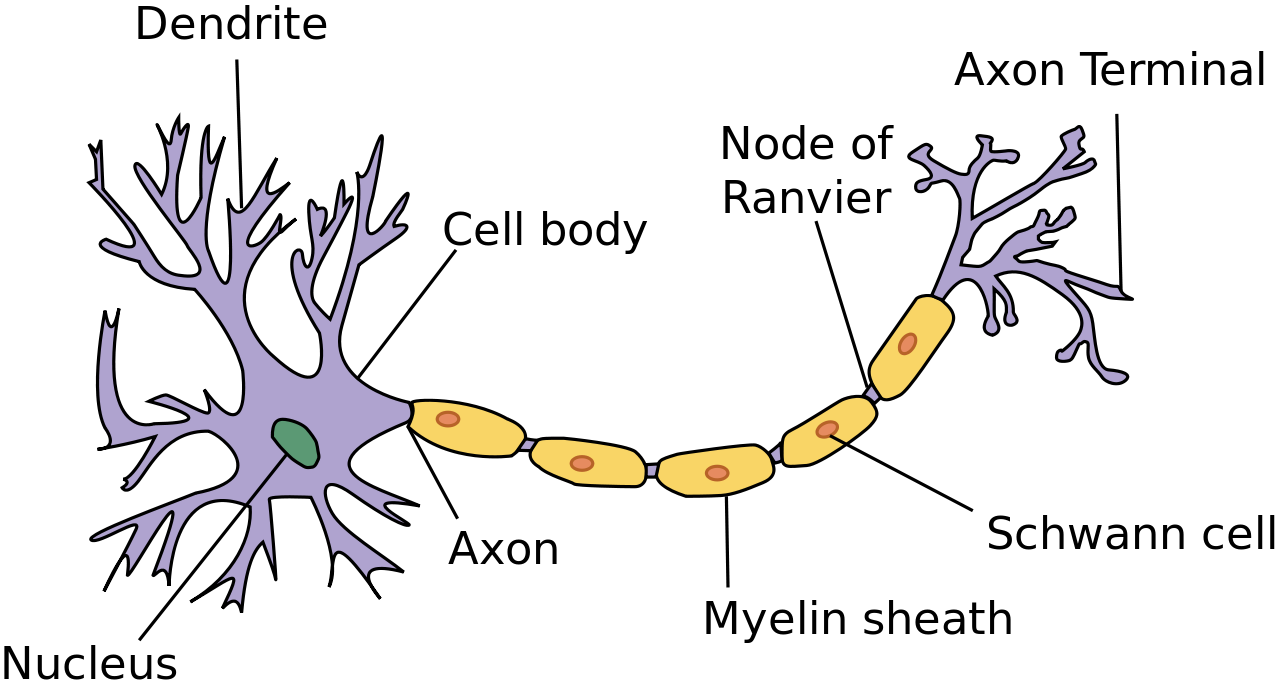
\includegraphics[scale=0.18]{charts/neuron.png}
				\caption{Cấu hình file hosts trên máy master}
				\label{fig:hosts}
			\end{figure}
			\textbf{Viết tiếp IP nào là master, IP nào là slave và chèn hình lại}
			
		\end{enumerate}
		
		\subsubsection{Truy cập SSH}
		SSH là giao thức mạng được sử dụng để đăng nhâp vào một máy tính từ xa. Hadoop sẽ sử dụng giao thức nay để kết nối các máy master và datanodes. Nhờ đó mà master có thể truy cập cũng như điều khiển các slaves.\par 
		Trong hduser của máy được chọn làm master ta lần thực hiện các lệnh sau để khai triển SSH.
		\begin{enumerate}
			\item Sinh ra cặp public key và private key
			\textbf{include graphic hình câu lệnh sshkeygen vào đây}
			\item Copy public key tới các máy slave đã được chọn
			\textbf{incude graphic các câu coppy id vào đây và giải thích}
			\item Kiểm tra thử kết nối đã thành công bằng cách:
			\textbf{include graphic hình kết nối thành công vô đây}
		\end{enumerate}
		
		\subsubsection{Cài đặt Hadoop}
			
			
		
				

	\subsection{Xử lý dữ liệu}
	
		Các hình ảnh được trình bày, dữ liệu được lưu vào các thư mục có chứa các tên mô tả cho đặt tính của những hình ảnh đó. Với bộ dữ liệu trên, chương trình tạo một kiểu dữ liệu dictionary với khóa chính là giá trị biểu diễn cho tên thư mục và cũng là tên class cần phân loại, value chính là đường dẫn các file ảnh tương ứng.\par
		 Để sử dụng được trong mô hình mạng, các hình ảnh sẽ được mã hóa sang một định dạng mới nhờ các phương thức hỗ trợ có sẵn trong thư viện Tensorflow. Sau khi được mã hóa, kết quả chính là các tensor có thông số shape như sau [299, 299, 3], với hai vị trí đầu tiên chính là kích thước của hình ảnh cũng như của tensor, giá trị 3 biểu diễn cho độ sâu (ảnh màu).\par
	 	Sau cùng, bộ dữ liệu đã được mã hóa được chia thành 3 tập con sử dụng với 3 mục đích khác nhau: tập huấn luyện(Training set), tập validation để tránh vấn đề overrfit trong quá trình huấn luyện và tập kiểm thử dùng để kiểm tra độ chính xác của mô hình sau khi huấn luyện hoàn tất.	Riêng tập huấn luyện sẽ được dùng để tạo ra các bottlenecks
	
	\subsection{Tạo các bottlenecks}
	
	Bottlenecks\cite{bottlenecks} là một từ được dùng để chỉ tầng (layer) nằm ngay trước fully-connected layer. Với kiến trúc mạng googLeNet, tầng này đã được huấn luyện tập dữ liệu trước đó nên có được kết quả đủ tốt để phân biệt được đặc tính của mỗi lớp(class) yêu cầu. Có nghĩa ở bước này chúng ta sẽ tạo ra một bản tóm tắt các giá trị trọng số đủ tốt cho mỗi ảnh input. Tầng cuối cùng của kiến trúc mạng sẽ sử dụng các giá trị bottlenecks này để huấn luyện và điều chỉnh để phân loại các lớp mới. Điều này nhờ vào việc mạng đã được huấn luyện bởi tập dữ liệu gồm 1000 lớp khác nhau của ImageNet giúp cho việc phát hiện các mẫu đặc tính trở nên dễ dàng hơn.
	
	\subsection{Huấn luyện}
	
	Sau khi hoàn tất tạo các giá trị bottleneck, việc thực hiện thực hiện cấu hình mạng và huấn luyện bắt đầu. Tổng số bước huấn luyện sẽ được cài đặt mặc định là 4000 bước, tuy nhiên có thể thay đổi lại tùy theo tình huống. Mỗi bước huấn luyện sẽ chọn ra 100 dữ liệu ngẫu nhiên \footnote{Tập dữ liệu lúc này là những bottlenecks} để đưa vào tầng cuối cùng \footnote{Tầng fully-connected với softmax là activation function} để dự đoán lớp, lớp dự đoán sẽ được so sánh với các lớp thực tế để mạng điều chỉnh và cập nhật các giá trị trọng số thông qua cơ chế lan truyền ngược như đã trình bày ở chương trước. Do phép toán được thực hiện trên tập huấn luyện nên sẽ  gây ra vấn đề overfit, vì thế mà tập validation sẽ được sử dụng để đo lại giá trị sai lệch và độ chính xác. Nếu độ chính xác tại tập huấn luyện cao nhưng tại tập validation không thay đổi hoặc thấp thì chứng tỏ mô hình mạng gặp phải vấn đề overfit và việc huấn luyện tiếp tục không còn có ích.
	


